\chapter{Hybrid Eulerian-Lagrangian Vortex Particle Method}
\label{ch:hybrid}
%\label{ch:LiteratureReview}

%\section{Eulerian-Lagrangian coupling algorithm}
%The hybrid coupling strategy that we used is a modification of the algorithms developed by Stock \cite{} and Daeninck \cite{}. The coupling scheme is simpler than the Schwarz alternating method, as it required no iteration for the coupling procedure. 
%\section{Theory of Domain Decomposition Method}
% Comparison of hybrid vortex methods.
% choice of hybrid method. Example domain decomposion, coupling technique
%\subsection{Advantage of domain decomposition}
%% What is the advantage?
%% What is the drawback?

Chapter \ref{ch:introduction} introduced the \printAcron{Hybrid Eulerian-Lagrangian Vortex Particle Method}{HELVPM}, a domain decomposition method, where the Eulerian method and the Lagrangian method are used to solve different domains of the fluid.  The algorithm that we use to couple the Lagrangian solver and the Eulerian solver is a modification of the procedures used by Stock and Daeninck. The algorithm is summarized as follows:

	\begin{enumerate}
	\item \textbf{Correct Lagrangian:} Use the solution of the Eulerian domain $\Omega_E$ (in the near-wall region) to correct the solution of the Lagrangian domain $\Omega_L$, that is overlapping the Eulerian domain.
	
	\item \textbf{Evolve Lagrangian:} With the modified solution, evolve the Lagrangian solution from time step $t_n$ to next time step $t_{n+1}$. Chapter \ref{ch:lagrangian} summarizes the procedures of evolving the Lagrangian solution.
	
	\item \textbf{Determine Eulerian boundary conditions:} Use the Lagrangian solution of time $t_{n+1}$ to determine the boundary conditions of the Eulerian domain at $t_{n+1}$.
	
	\item \textbf{Evolve Eulerian:} With the boundary condition, evolve the Eulerian solution from $t_n$ to $t_{n+1}$. Chapter \ref{ch:eulerian} summarizes the procedures of evolving the Eulerian solution.
	\end{enumerate}

We dedicated the chapter \ref{ch:lagrangian} to give an overview on the implementation of the Lagrangian solver. The Lagrangian domain consists of vortex panels that represents the wall-bounded vorticity, and vortex blobs that represents the vorticity everywhere else in the fluid. Chapter \ref{ch:eulerian} was dedicated to introduce the implementation of the Eulerian solver. We decided to use a Finite Element solver that models an incompressible laminar flow using velocity-pressure $\mathbf{u}-p$ formulation. The domain of the Eulerian method is bounded to the body and is used to simulate the vorticity generation from no-slip boundary.

In this chapter, we will elaborate on the coupling of the Eulerian solver and the Lagrangian solver (steps 2 \& 4) to construct the Hybrid Eulerian-Lagrangian Vortex Particle Method. 

\section{Decomposition of the domain}
The hybrid scheme consists  of the decomposition the domain into two subdomains. Figure \ref{fig:hybrid_domains} shows the segregation of the fluid to the near-wall region $\Omega_E$, where an Eulerian solver is used to resolve the near-body region, and a Lagrangian solver is used to resolve the wake region $\Omega_L$.
	\begin{figure}[h]
	\centering
	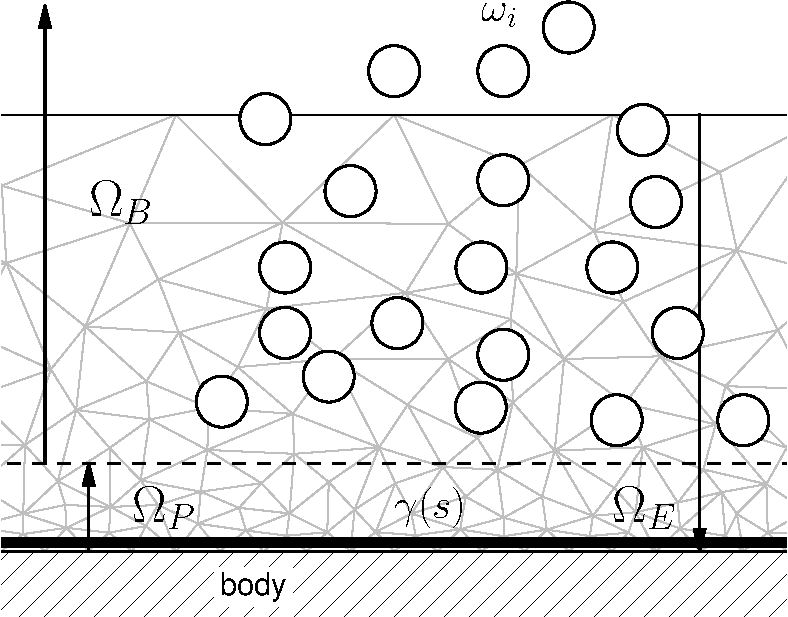
\includegraphics[width=0.45\linewidth]{./figures/hybrid/interpolation/hybrid_domains-crop.pdf}
	\caption{Schematic of the hybrid domain with the Lagrangian domain $\Omega_L: \Omega_P \cup \Omega_B$ and the Eulerian domain $\Omega_E$ resolving the near-wall region $\Omega_E: \Omega_E \subset \Omega_L$.}
	\label{fig:hybrid_domains}
	\end{figure}

The Lagrangian domain $\Omega_L$ is divided into two subdomain: the domain $\Omega_B$ of the vortex blob $\omega(\mathbf{x},t): \mathbf{x} \in \Omega_B$; and the domain $\Omega_P$ of the wall-bounded vortex panel $\gamma(\mathbf{\hat{s}}) \in \Omega_{P}$, the vortex panel domain. In section \ref{sec:boundaryConditions}, we saw that in order to deal the singular wall-bounded vortex sheet distribution, we require a kernels that can represent such distribution. Therefore, the decomposition of the domain is as follows:

	\begin{equation}
	\textit{fluid}:\quad\begin{cases}
	\Omega_E, &\qquad \text{(\textit{Eulerian domain})}  \\
	\Omega_L: \Omega_{P} \cup \Omega_B, &\qquad \text{(\textit{Lagrangian domain})}
	  \end{cases}
	\end{equation}

with the requirements on the domains that:
	\begin{itemize}
	\item Eulerian domain resolves the near-wall region of the Lagrangian domain, $\Omega_E \subset \Omega_L$,
	\item Vortex panel domain is bounded to the wall boundary of the Eulerian domain, $\Omega_P \subset \Omega_E$
	\item Vortex blob domain does not overlap with the vortex panel domain, $\Omega_B \cap \Omega_P : \varnothing$
	\end{itemize}

During the decomposition of the domain, we defined three boundaries, figure \ref{fig:hybrid_config}:
\begin{itemize}
\item No-slip wall boundary of the Eulerian and the vortex panel domain, $\partial \Omega_{\mathrm{wall}}$
\item External boundary of the Eulerian domain where we will prescribe the Dirichlet velocity boundary condition, $\partial \Omega_{E}$.
\item The boundary of the vortex panel domain $\Omega_P$ and the vortex blob domain $\Omega_B$, $\partial \Omega_P$.
\end{itemize}	

	\begin{figure}[t]
	\centering
	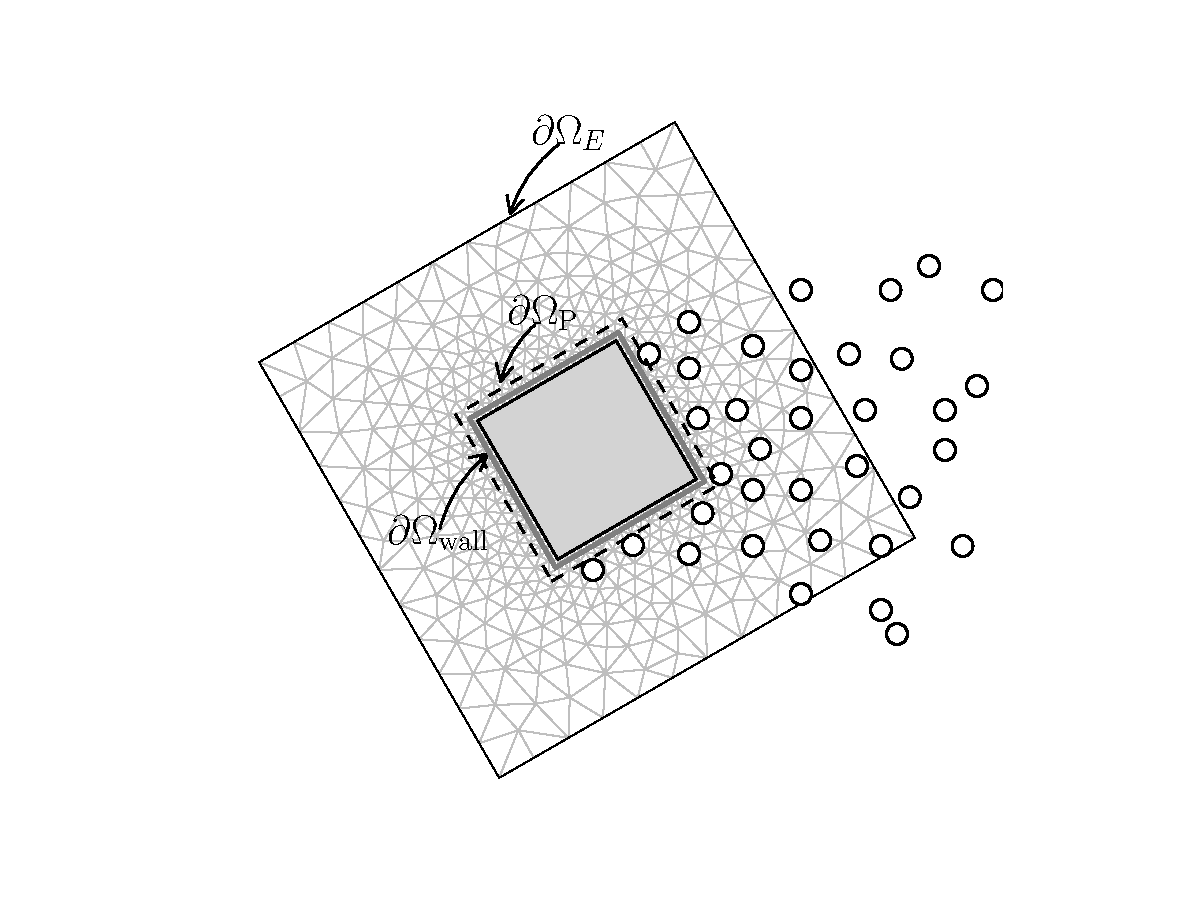
\includegraphics[trim=3.9cm 1.6cm 3.3cm 1.6cm, clip,  width=0.5\linewidth]{./figures/hybrid/interpolation/hybrid.pdf}
	\caption{Boundaries of the hybrid domain}
	\label{fig:hybrid_config}
	\end{figure}	
	%trim=4.37cm 1.58cm 3.86cm 1.58cm, clip,

The coupling of the Eulerian solver and the Lagrangian solver is performed by coupling the solutions of the overlap region $\Omega_E \cap \Omega_L$ according to the procedure of Stock and the Daeninck.

\subsection{Local to Global Transformation}

The geometries in the simulation are defined in their respective coordinate system, $[x,y]'$. Figure \ref{fig:localPosition} shows an elliptical geometry defined in its local coordinate system about its origin $[{x_o},{y_o}]'$. The origin point is defined such that it is the center of rotation. For a typical airfoil, we will have $[x_o,y_o]' = [c/4,0]$, pitching the airfoil by $\theta_{local}$ about the quarter-chord point.

	\begin{figure}[h]
     \centering
     \begin{subfigure}[t]{0.45\textwidth}
             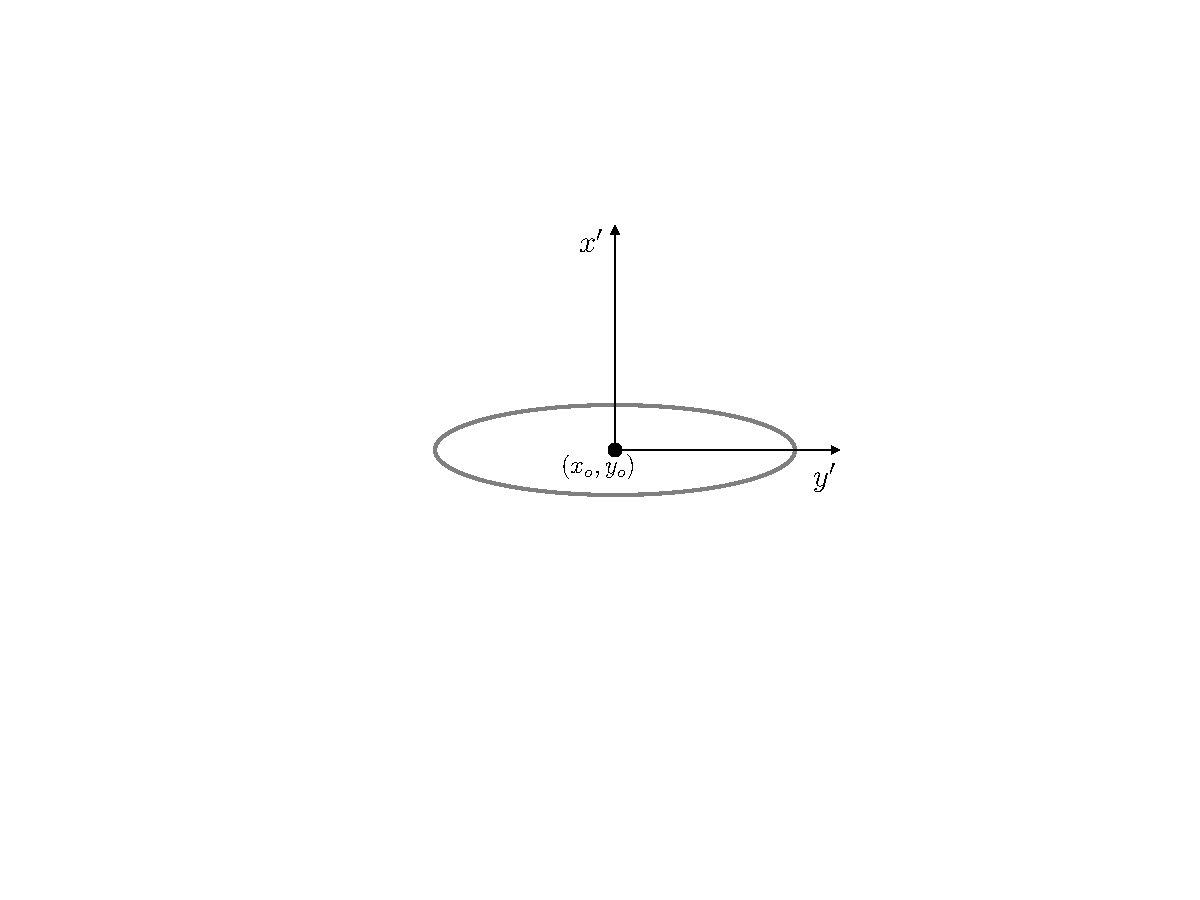
\includegraphics[trim=4.5cm 2.cm 3.5cm 1.5cm, clip, width=\linewidth]{./figures/hybrid/interpolation/ellipse/localOrientation.pdf}
             \caption{Loc}
             \label{fig:localPosition}
     \end{subfigure}%
     ~ %add desired spacing between images, e. g. ~, \quad, \qquad etc.
       %(or a blank line to force the subfigure onto a new line)
     \begin{subfigure}[t]{0.45\textwidth}
             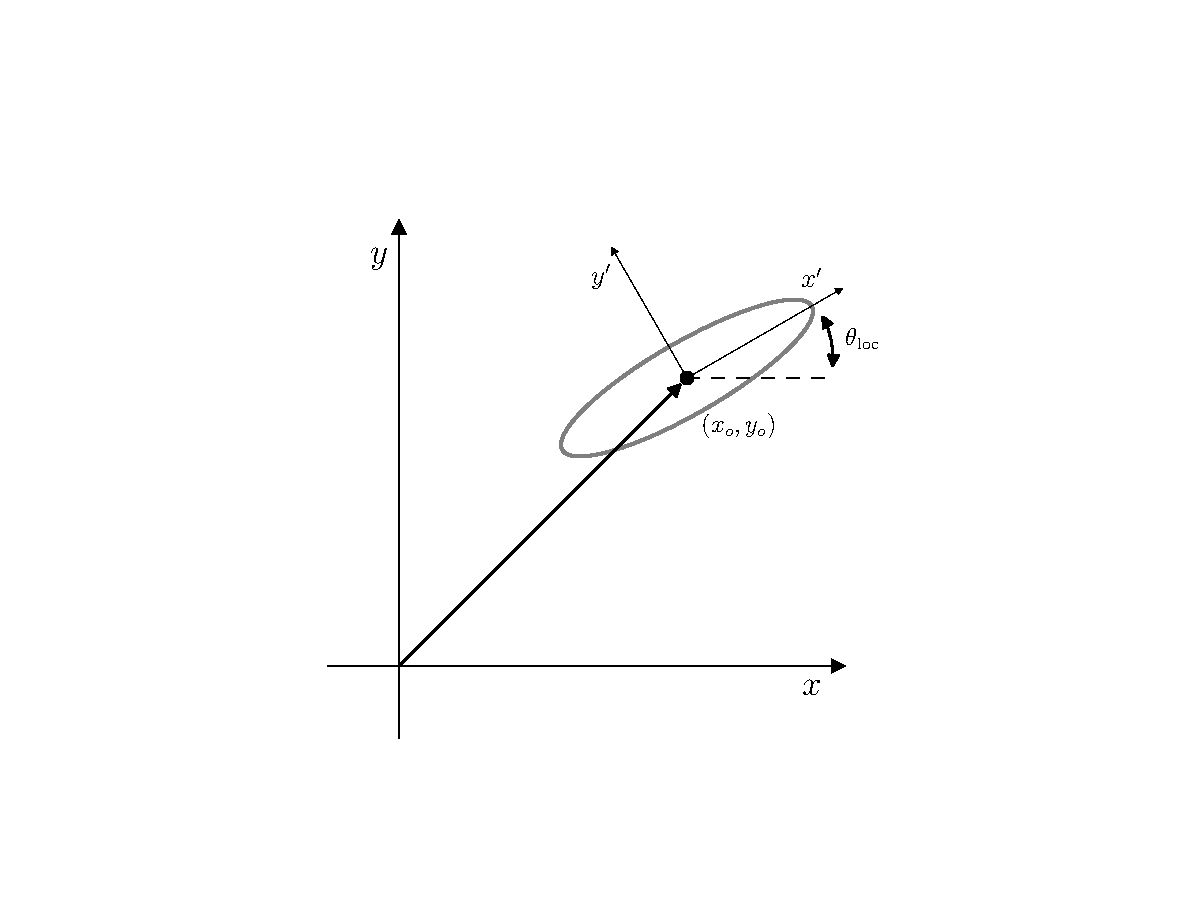
\includegraphics[trim=4.5cm 2.cm 3.5cm 1.5cm, clip, width=\linewidth]{./figures/hybrid/interpolation/ellipse/globalOrientation.pdf}
             \caption{Glob}
             \label{fig:globalPosition}
     \end{subfigure}

     \caption{Orientation}
     \label{fig:positionOfBody}
	\end{figure}
	
The body is then transformed to the global coordinate system $[x,y]$ by the displacement vector $[x_o,y_o]$ and a local rotation by $\theta_{\mathrm{loc}}$ about the local origin $[x_o,y_o]$. 

The Eulerian solver defines the body mesh in the local coordinate system is then transformed to global position using these parameters. Similarly, the panel geometry for the Lagrangian solver is defined in the same fashion. For a moving problems, the displacement vector and the local rotation angle can be updated to prescribe the motion.


\section{Correction of Lagrangian domain}

The first step of the hybrid coupling scheme is to transfer the highly resolved Eulerian solution to the Lagrangian domain. This is performed by transferring the vorticity in the Eulerian domain $\Omega_E$ onto the vortex blobs that are inside the Eulerian region, $\mathcal{P}: \mathcal{P} \in \Omega_E \cap \Omega_B$.
				
\subsection{Approach from literature}		
							
However, as Stock has described \cite{} and shown by Daeninck in figure \ref{fig:daeninck_CylinderVorticity}, the Eulerain solution is assumed to be correct from the body up to ``somewhat inside of the outer Eulerian domain", and the Lagrangian solution is valid outside of the outer Eulerian boundary. 

	\begin{figure}[h]
	\centering
	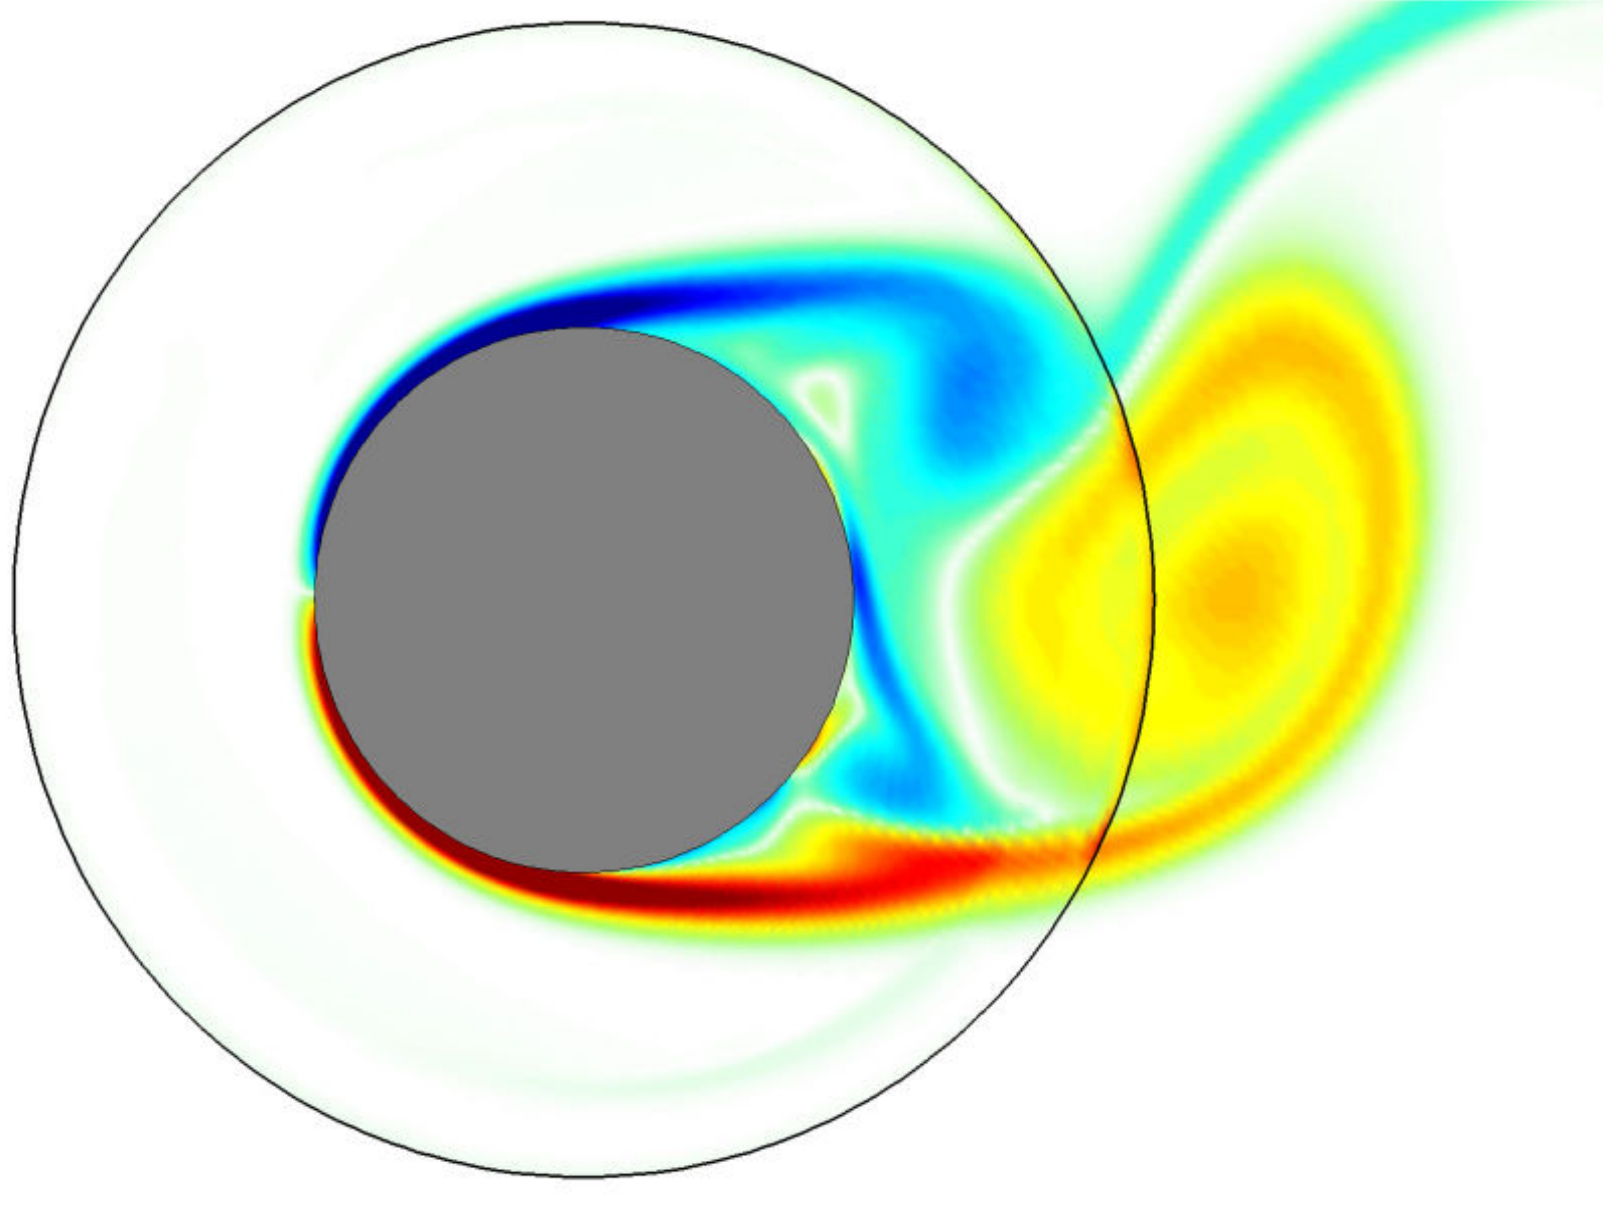
\includegraphics[width=0.5\linewidth]{./figures/hybrid/daeninck_CylinderVorticity.png}
	\caption{Daeninck artificial vorticity at the boundary}
	\label{fig:daeninck_CylinderVorticity}
	\end{figure}

At the boundary of the Eulerian boundary $\partial \Omega_E$, the figure \ref{}, shows artificial vorticity due to slight difference in the solution. To overcome this problem, Stock proposed to interpolate only part of the Eulerian domain onto the Lagrangian domain, as shown in figure \ref{fig:interpRegion}. The interpolation region $\Omega_{int}$ ignores the boundary layer region with the very strong vorticity gradients (which will be resolved by the vortex panel), and part of the outer Eulerian boundary where the Eulerian solution is less accurate. So the interpolation region has the following properties:

	\begin{itemize}
	\item The domain is within the overlap region, $\Omega_{int} \subseteq \Omega_E \cap \Omega_B$,
	\item The domain is bounded by the boundary $\partial \Omega_P$ near the wall with an offset of $d_{surf}\cdot h$ from the surface $\partial \Omega_{\mathrm{wall}}$.
	\item The domain is bounded by the boundary $\partial \Omega_{int}$ at the outer boundary with an offset of $d_{bdry}\cdot h$ from the outer Eulerian boundary $\partial \Omega_{E}$.
	\end{itemize}

	\begin{figure}[t]
     \centering
     \begin{subfigure}[t]{0.35\textwidth}
             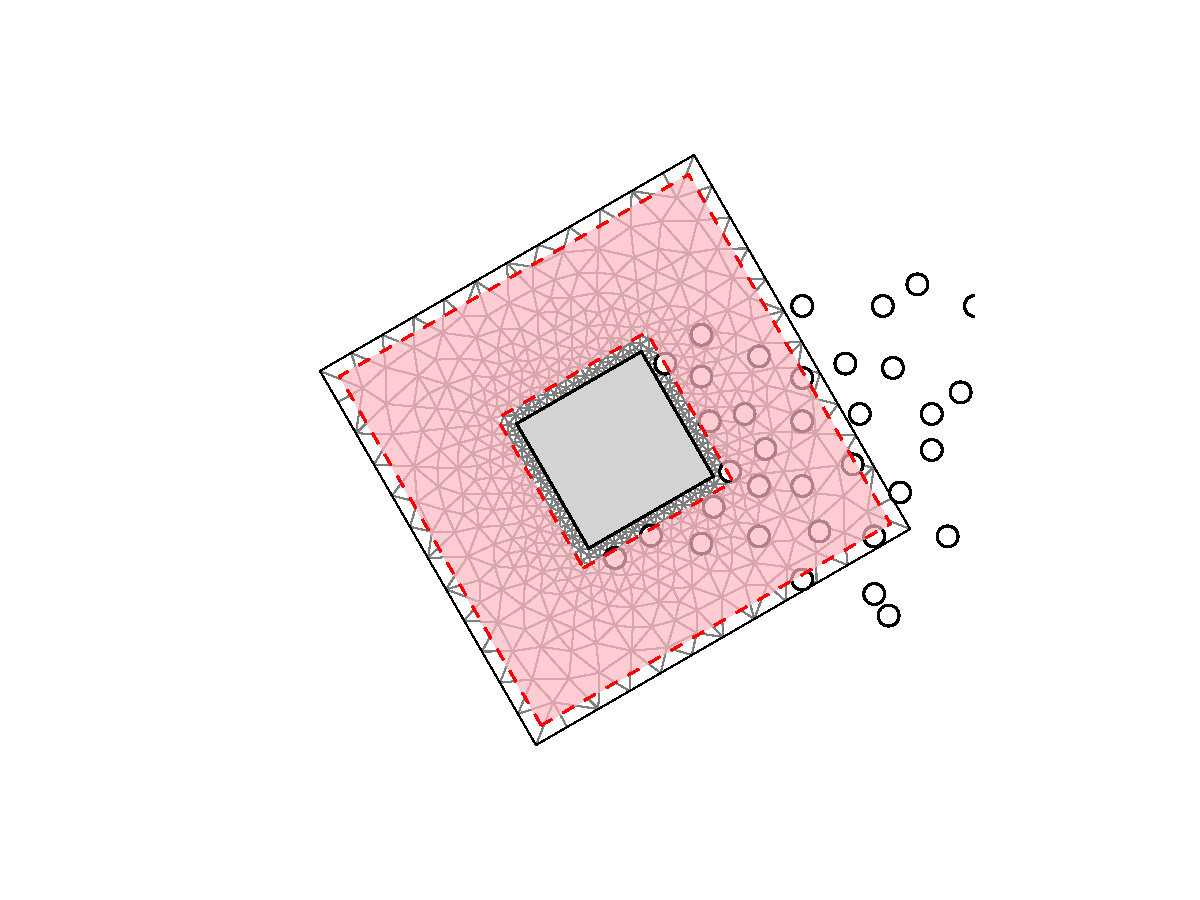
\includegraphics[trim=4.37cm 1.58cm 3.86cm 1.58cm, clip, width=\linewidth]{./figures/hybrid/interpolation/interpRegion.pdf}
             \caption{interpolation region}
             \label{fig:interpRegion}
     \end{subfigure}%
     ~ %add desired spacing between images, e. g. ~, \quad, \qquad etc.
       %(or a blank line to force the subfigure onto a new line)
     \begin{subfigure}[t]{0.6\textwidth}
             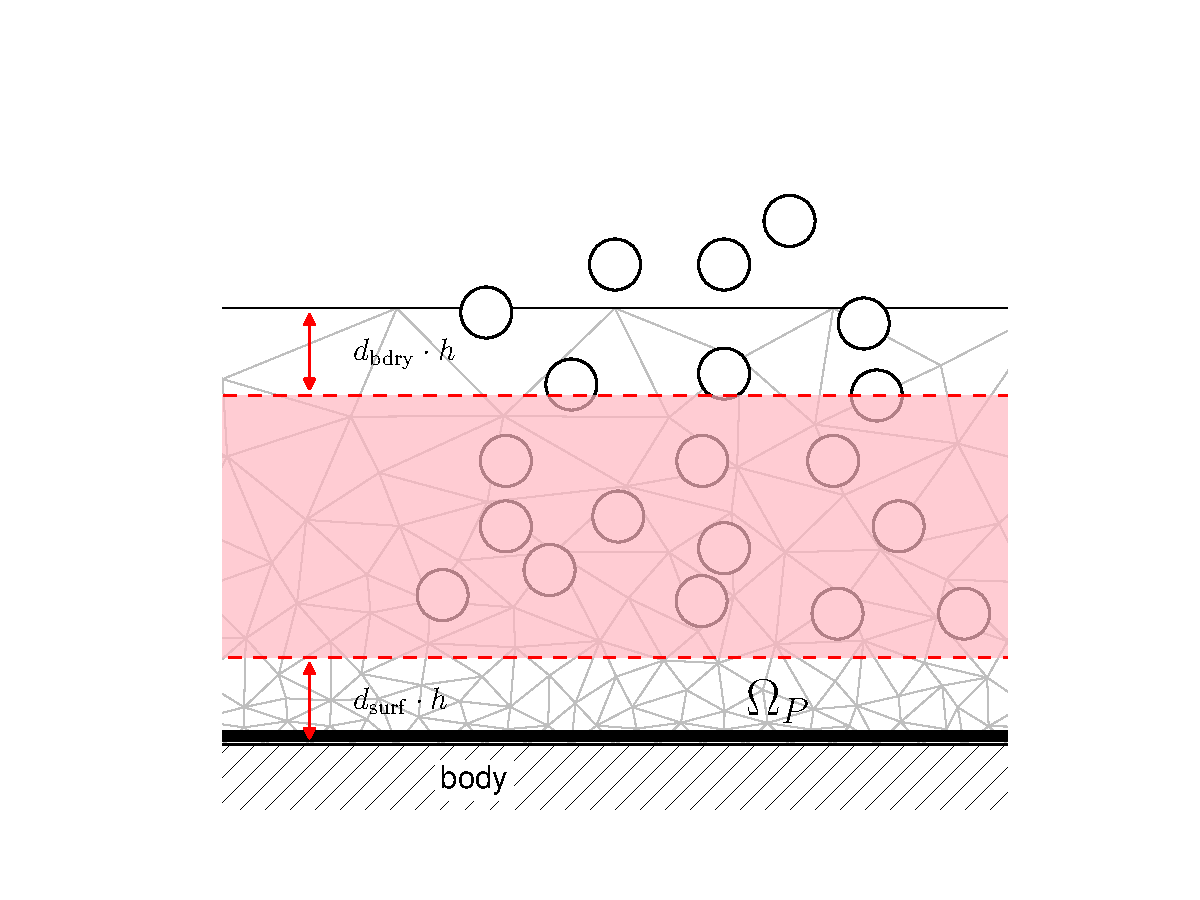
\includegraphics[width=\linewidth]{./figures/hybrid/interpolation/hybrid_domains_withInterpReg.pdf}
             \caption{Interpolation regions}
             \label{fig:hybrid_domains_withInterpReg}
     \end{subfigure}

     \caption{Interp regigs}
     \label{fig:interpolationRegionDefinitions}
	\end{figure}	

The summary of the interpolation algorithm for transferring the Eulerian solution to the vortex blobs used by Stock based on work of Daeninck and Guermond \& Lu is as follows:
\begin{enumerate}
\item Interpolate the solution from Eulerian domain onto a temporary structured grid. Ignore very strong vorticity at the boundary layer, $\mathbf{x} \in \Omega_P$.
\item Determine the locations of the particles inside the interpolation region $\Omega_{int}$. Fill gaps in the region with zero-strength particles. 
\item Reset the strengths of the particles $\mathbf{x}_i$ inside the interpolation region $\Omega_{int}$, figure \ref{fig:interpRegion}, using the local particle volume and the vorticity interpolated from the grid (i.e $\alpha_i = \omega_i\cdot{h^2}$).
\end{enumerate}

Though, through our research we have determined that this approach suffers from issues and does not guarantee the conservation of circulation. 

\subsection{Issues with the correction algorithm}

The two main issues with the above approach is as follows:

\begin{itemize}
\item The vorticity bounded to the solid wall was not interpolated to the vortex blobs. 
\item The second issue is that the particle strengths are initialized using standard cell circulation equation, $\alpha_i = \omega \cdot h^2$. This is the standard approach used by the vortex particle community however, this method does not ensure accurate interpolation of the vorticity field, as described by Barba \& Rossi \cite{Barba2010a}.
\end{itemize}

\subsubsection{Vorticity at the solid wall}

%Therefore to overcome this issue we propose to prescribe the total circulation of the panels such that the circulation is conserved globally.

%\subsubsection*{Prescribed panel strengths}


The first problem that we are concerned is that the vorticity bounded at the solid wall was not transfered to the Lagrangian domain. This is especially problematic in our case as the vortex panel that we have implemented does not diffuse their strength to the vortex blobs. We have implemented the approach used by Daeninck, where the vorticity generated at the wall boundary is introduced from the Eulerian domain. 

To ensure that circulation is conserved, the circulation in the vortex panel domain $\Omega_P$ must be somehow introduced to the Lagrangian domain. Furthermore, if the geometry is at motion, the body itself will have circulation due to the rotation, given as:
	\begin{equation}
	\Gamma_{\mathrm{body}} = \iint\limits_{\mathrm{body}} \nabla \times \mathbf{u}_b \ d A.
	\end{equation}

Therefore, in order to ensure conservation of the circulation, we proposed to transfer the circulation of the domain $\Omega_P$ and the circulation inside the body $\Omega_{\mathrm{body}}$ to the panels.


\subsubsection{Vorticity Field interpolation error}
	
The second issue we must tackle is the interpolation error that arises due to the standard approach of initializing the particles using the local particle volume and the local vorticity,
	\begin{equation}
	\alpha_i = \omega_i\cdot{h^2},
	\end{equation}
where $i$ corresponds to the vortex blobs $\mathbf{x}_i \in \Omega_{int}$. We summarized this issue in the section \ref{} of the Lagrangian chapter and was extensively investigated by Barba \& Rossi \cite{Barba2010a}. To solve the wake domain of the fluid, we used a vortex particle method that discretizes the vorticity field using $N$ quadrature points,
\begin{equation}
\omega \approx \omega^h(\mathbf{x}_j) = \sum_{i=1}^N \alpha_i \delta(\mathbf{x}_j - \mathbf{x_i}).
\end{equation}

We smoothed the singular kernel $\delta$ by using a Gaussian kernel $\zeta_{\sigma}$. This approach of using vortex blobs is common in the field of vortex particle method and ensures smooth vorticity field. However, the downside to this approach is that on top of the discretization error, we know introduce a so called ``smoothing error" or the ``regularization error" due to the use of gaussian kernel. This is equivalent to blurring the vorticity field, as explained by Barba \& Rossi \cite{Barba2010a}, and the cumulative error in the initialization error is given as

\begin{equation*}
\mathrm{Initialization\ Error} = \mathrm{Smoothing\  Error} + \mathrm{Discretization\ Error}
\end{equation*}

To perform accurate interpolation of the vorticity $\omega$ inside the interpolation domain $\Omega_{int}$ onto the particles $\mathbf{x}_j \in \Omega_{int}$, we must satisfy the following interpolation problem:
	\begin{equation}
	\omega(\mathbf{x}_j) = \hat{\omega}(\mathbf{x}_j),
	\end{equation}
where
	\begin{equation}
	\hat{\omega}(\mathbf{x}) = \sum_{i=1}^{N} \alpha_i \zeta_{\sigma}(\mathbf{x}_j - \mathbf{x}_i),
	\end{equation}
is the discrete vorticity field represented by the linear combinations of the gaussian basis function $\zeta_{\sigma}$ with the vortex blob strength $\alpha_i$. Therefore, assuming the $\alpha_i = \omega(\mathbf{x}_i)\cdot{h^2}$ is incorrect.

As discussed in the secion \ref{} of the Lagrangian chapter, one would assume that the strengths of the particles can be determined by solving the following linear system of equations:
\begin{equation}
\mathbf{A}_{ij}\alpha_i = \omega_i,
\end{equation}
where 
\begin{equation}
\mathbf{A}_{ij} = \zeta_{\sigma}(\mathbf{x}_j-\mathbf{x}_i).
\label{eq:initialization}
\end{equation}

However inverting the matrix $\mathbf{A}$ is still an open question, as stated by Koumoutsakos \& Cottet \cite{}. The problem is that the matrix $\mathbf{A}$ is full and badly condition for direct inversion. For a global field interpolation (i.e for unbounded domain), one could use the Beale's iterative method which uses a \printAcron{successive over-relaxation}{SOR} for solving the equation \ref{eq:initialization}. This method relies on iterative correction of all the particles $\mathbf{x}_i \in \Omega_L$, the Lagrangian domain. 

In our case of initializing the strengths of the particles $\mathbf{x}_i$ in the sub-domain $\Omega_{int}$, it would require us to modify the strength of all the particles $\mathbf{x}_i$ in all $\Omega_B$. This is not feasible not feasible as the size of the problem is very large when the wake is fully developed ($10^5 \leqslant N_{\mathrm{blobs}}$).

Therefore, currently the best possible way of ensure minimal interpolation error from Eulerian domain onto vortex blobs is to perform the following steps:
\begin{itemize}
\item Minimize the smoothing and discretization error by maximizing the particle resolution, achieved by setting $Ov=1$ and reducing $\sigma$ such that the relative error $\epsilon \leqslant 5\%$.
\item As conservation of circulation is a key requirement in fluid dynamic simulation, we ensure that conservation of circulation is not violated when initializing the particles inside the domain $\Omega_{int}$.
\end{itemize}


\subsection{Modified correction strategy}

The modified version of the correction can be divided into five sub-steps
\begin{enumerate}
\item \textbf{Probe vorticity}: Interpolate the vorticity from the Eulerian finite element space onto a uniform structured grid.
\item \textbf{Remove particles}: Remove particles that are inside the interpolation domain $\Omega_{int}$.
\item \textbf{Generate particles}: Generate zero-strength particle inside 
\item \textbf{Assign strengths}: Using the local volume and sldada.. assign the strength of the particles
\item \textbf{Conserve circulation}: Determine the mismatch in the total circulation of the Lagrangian field as determine the strength of the panels such that circulation is conserved.
\end{enumerate}

\subsubsection*{Probe vorticity}

The first sub-step of the correction step is to interpolate the vorticity from the unstructured Eulerian grid onto a uniform structured grid. The purpose of the structured grid is to perform fast and efficient interpolation of vorticity from the Eulerian domain onto the vortex blobs. 

	\begin{figure}[h]
	\centering
	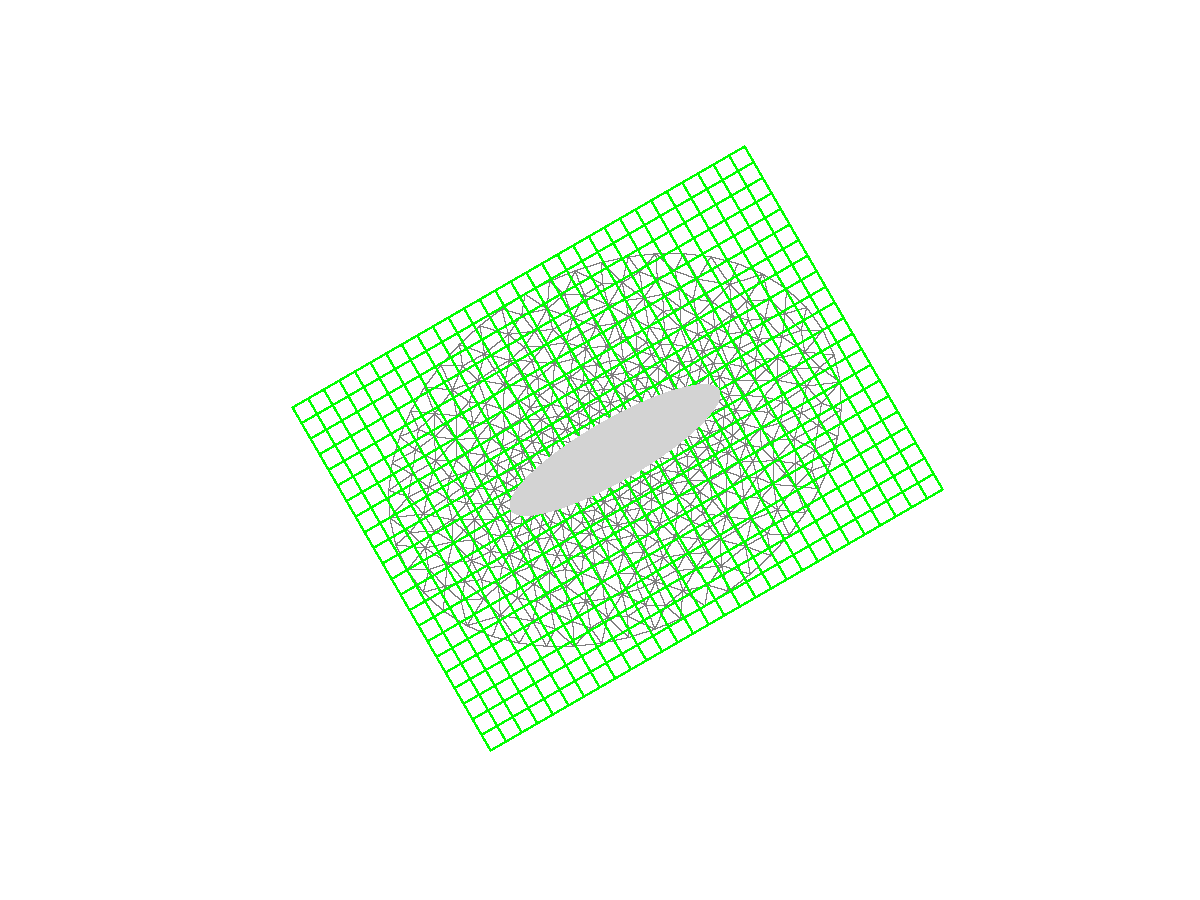
\includegraphics[trim=4.37cm 1.58cm 3.86cm 1.58cm, clip, width=0.5\linewidth]{./figures/hybrid/interpolation/ellipse/interpolation_FE2andStructuredGrid.pdf}
	\caption{Structured interpolation grid $\mathbf{x}_{str}$ covering the Eulerian domain $\Omega_E$.}
	\label{fig:interpolation_FE2andStructuredGrid}
	\end{figure}	
	
The structured grid $\mathbf{x}_{str}$ is defined in the local coordinates system of the geometry $[x,y]'$ where the grid covers the entire Eulerian domain $\Omega$. Figure \ref{fig:interpolation_FE2andStructuredGrid} shows the structured grid bounded to the Eulerian domain in the global coordinate system. The structured grid is bounded to Eulerian domain in the global coordinates system and is transformed with the same displacement vector and the rotation angle as the geometry. 

The vorticity function $\omega$ of the function space $X$ is interpolated from the unstructured mesh $\mathbf{x}_{\mathrm{unstr}}$ onto the structured uniform grid $\mathbf{x}_{\mathrm{str}}$,
	\begin{eqnarray}
	\hat{\omega}_i = \sum_k \omega_k W_{ki}
	\end{eqnarray}
using the interpolation weight $W$, giving us the structured vorticity field $\hat{\omega}$. As the structured grid $\mathbf{x}_{\mathrm{str}}$ that does not move w.r.t to the unstructured mesh $\mathbf{x}_{\mathrm{unstr}}$, the interpolation weight $W$ only needs to be calculated. 

After we have determined the vorticity $\hat{\omega}$, we assign the strengths of the particles using an efficient index search algorithm. If we were to transfer the vorticity directly from the unstructured mesh onto the vortex blobs, at each iteration, we would require an expensive search algorithm to determine the position of the blob w.r.t to the nodes of the unstructured grid. This would mean that we would have to construct the interpolation matrix at each iteration, drastically reducing the efficiency of interpolation.

	\begin{figure}[h]
	\centering
	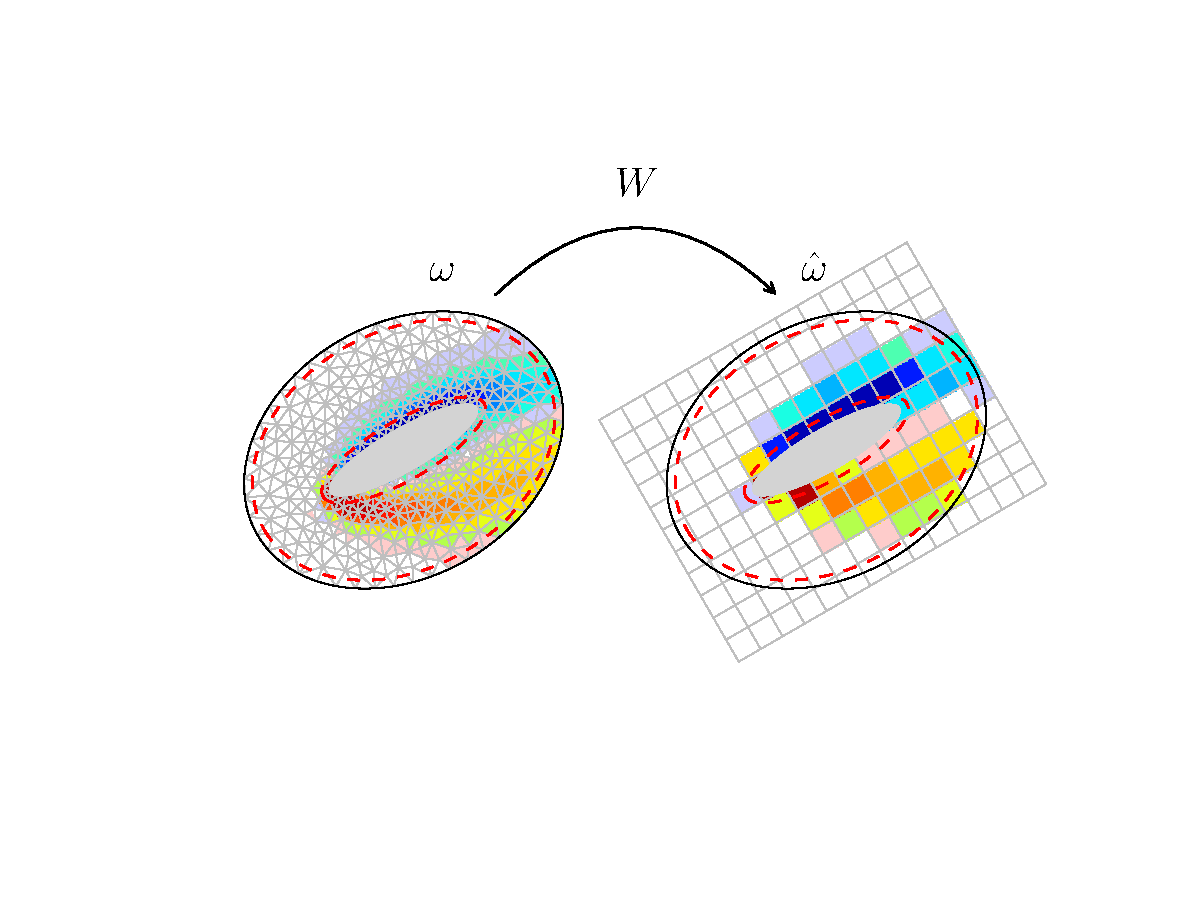
\includegraphics[trim=4.cm 4cm 2cm 2.5cm, clip, width=0.7\linewidth]{./figures/hybrid/interpolation/ellipse/interpolation_FE2StructuredGrid_withData.pdf}
	\caption{Interpolated vorticity $\hat{\omega}$ on the structured grid $\mathbf{x}_{str}$ from interpolating $\omega$ of the unstructured grid $\mathbf{x}_{unstr}$ with the interpolation weights $W$.}
	\label{fig:interpolation_FE2StructuredGrid_withData}
	\end{figure}

We used the \texttt{Probe} function, a fast C++ implementation developed by Mortensen \cite{fenicstools}, to the probe the vorticity function space $X$ for the structured vorticity $\hat{\omega}$.


\subsubsection*{Remove particles}

	\begin{figure}[h]
     \centering
     \begin{subfigure}[t]{0.49\textwidth}
             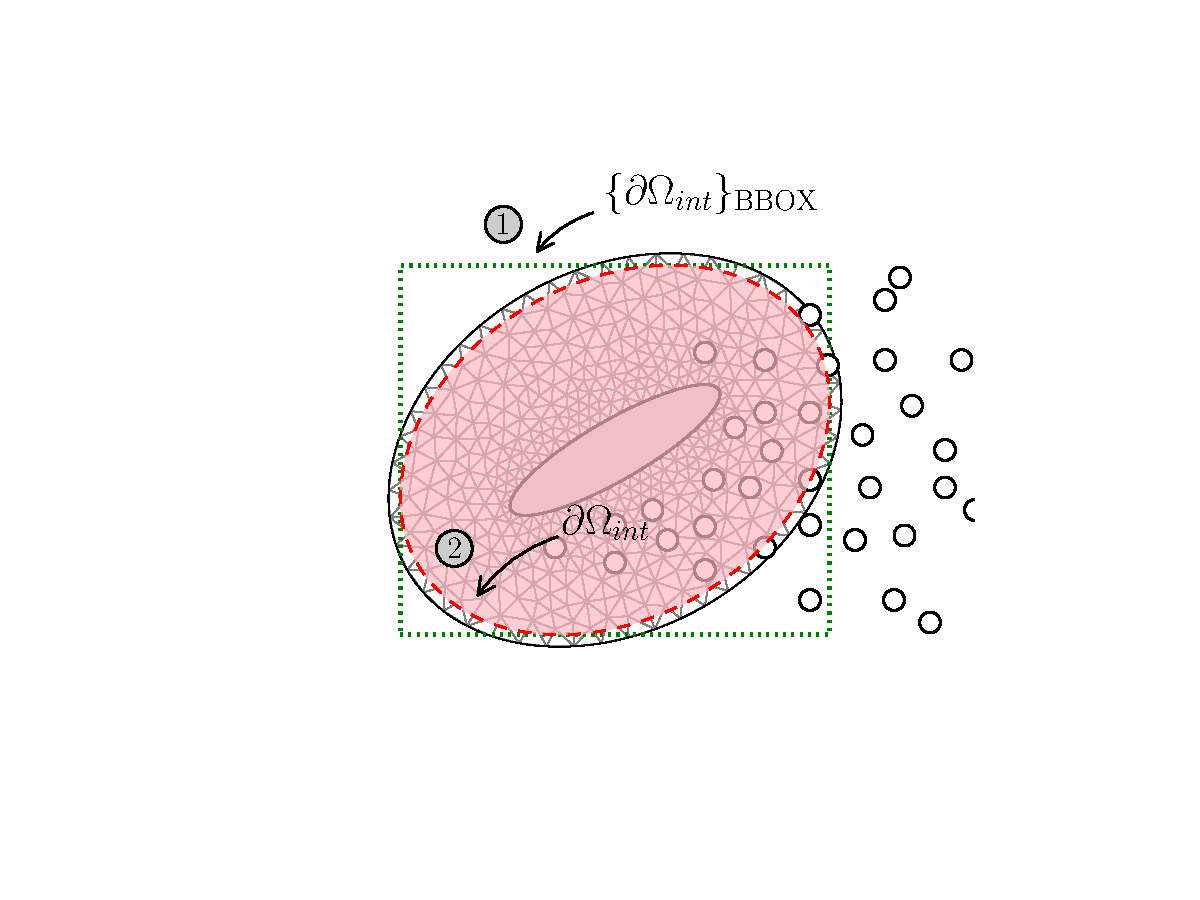
\includegraphics[trim=4.37cm 1.58cm 3.86cm 1.58cm, clip, width=\linewidth]{./figures/hybrid/interpolation/ellipse/interpRegion.pdf}
             \caption{Particles inside the interpolation region}
             \label{fig:region}
     \end{subfigure}%
     ~ %add desired spacing between images, e. g. ~, \quad, \qquad etc.
       %(or a blank line to force the subfigure onto a new line)
     \begin{subfigure}[t]{0.49\textwidth}
             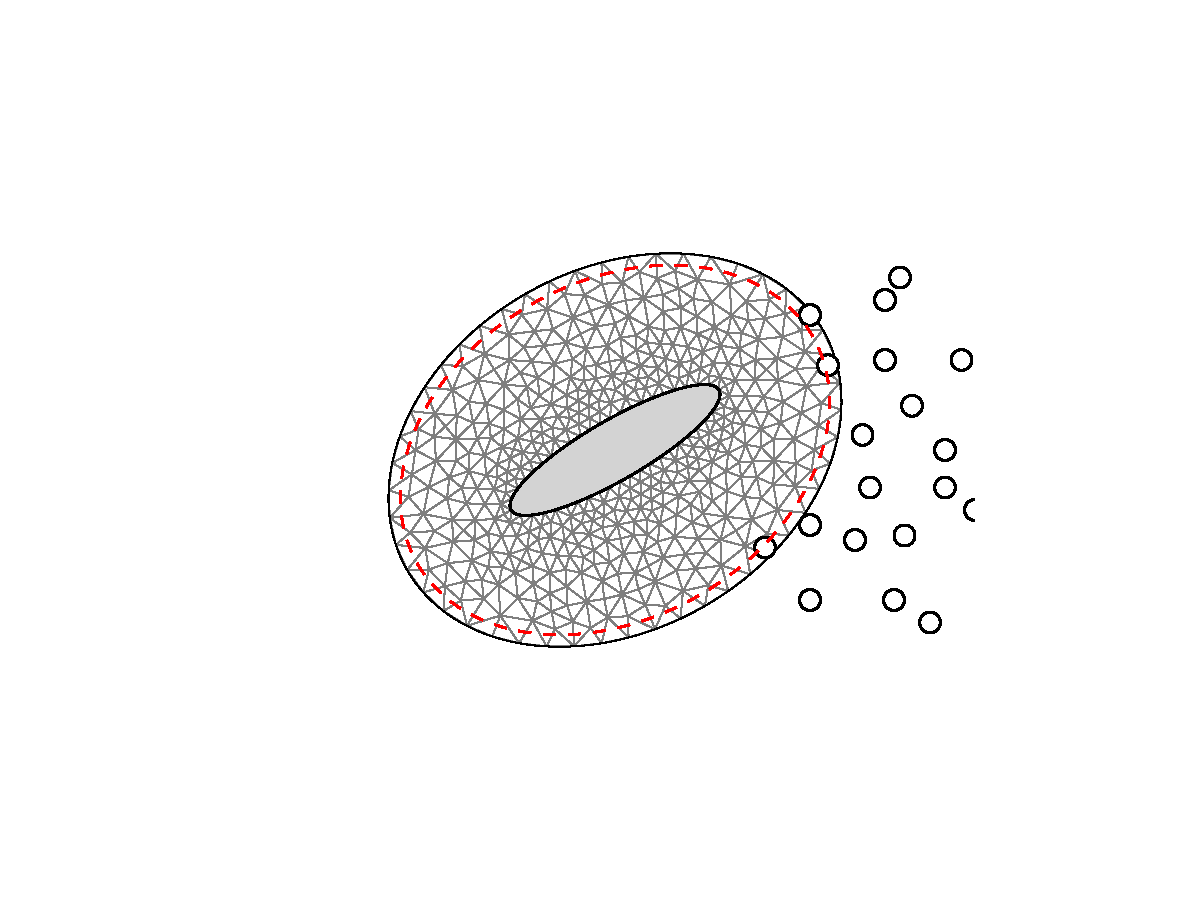
\includegraphics[trim=4.37cm 1.58cm 3.86cm 1.58cm, clip, width=\linewidth]{./figures/hybrid/interpolation/ellipse/particleRemoved.pdf}
             \caption{Total circulation $\Gamma_{rem}$ removed.}
             \label{fig:removed}
     \end{subfigure}

     \caption{The interpolation region $\Omega_{int}$, bounded by the boundary polygons: panel region boundary $\partial \Omega_P$ near the wall, and exterior boundary $\partial \Omega_{int}$ near the outer region.}
     \label{fig:interpRegionEllipse}
	\end{figure}	

The second sub-step of the correction step is remove the particles that are inside the interpolation region $\Omega_{int}$ and the vortex panel domain $\Omega_p$. The purpose of this step is that we want to ultimately correct the Lagrangian solution in these regions with the more refined Eulerian solution of the domain $\Omega_E$. To perform the coupling, we need to remove the particles in the region of correction $\Omega_{int}$ and $\Omega_p$. Figure \ref{fig:region} shows the vortex blobs $\mathbf{x}_b$ inside the boundary $\partial \Omega_{int}$ that needs to be removed. 

In order to determine if the particles are inside, we need to perform a ``Point inclusion in polygon" test to determine if the particle $\mathbf{x}_i$ is within the boundary polygon $\partial \Omega_{int}$. However, this point-in-polygon search is expensive and can be simplified by neglecting the particles outside the minimum bounding box of the polygon. The steps to remove the vortex blobs are as follows:
\begin{enumerate}
\item Determine the particles inside the bounding box of the polygon $\partial \Omega_{int}$. 
\item Perform a point-in-polygon test for only the particles $\mathbf{x}_i \in \mathrm{BBOX}\{\partial \Omega_{int}\}$.
\item Remove particles $\mathbf{x}_i$ from the total set of particles, resulting in a total circulation change of $\Gamma_{removed}$.
\end{enumerate}

To perform the point-in-polygon test, we used the \texttt{pnpoly} function of \texttt{matplotlib}, the python 2D plotting library created by Hunter \cite{Hunter:2007}. The function implemented the ``point inclusion in polygon" test algorithm developed by Franklin \cite{franklin2006pnpoly}. The algorithm is based on the crossings test, which determines if the point is inside the polygon by determining the number of the time a semi-infinite ray originating from the point intersects with the polygon.

\subsubsection*{Generate particles}

The third sub-step of the correction step is generate zero-strength particles inside interpolation region $\Omega_{int}$. This zero-strength particles will later be corrected with the strengths obtained from the structured grid $\mathbf{x}_{str}$.

	\begin{figure}[h]
	\centering
	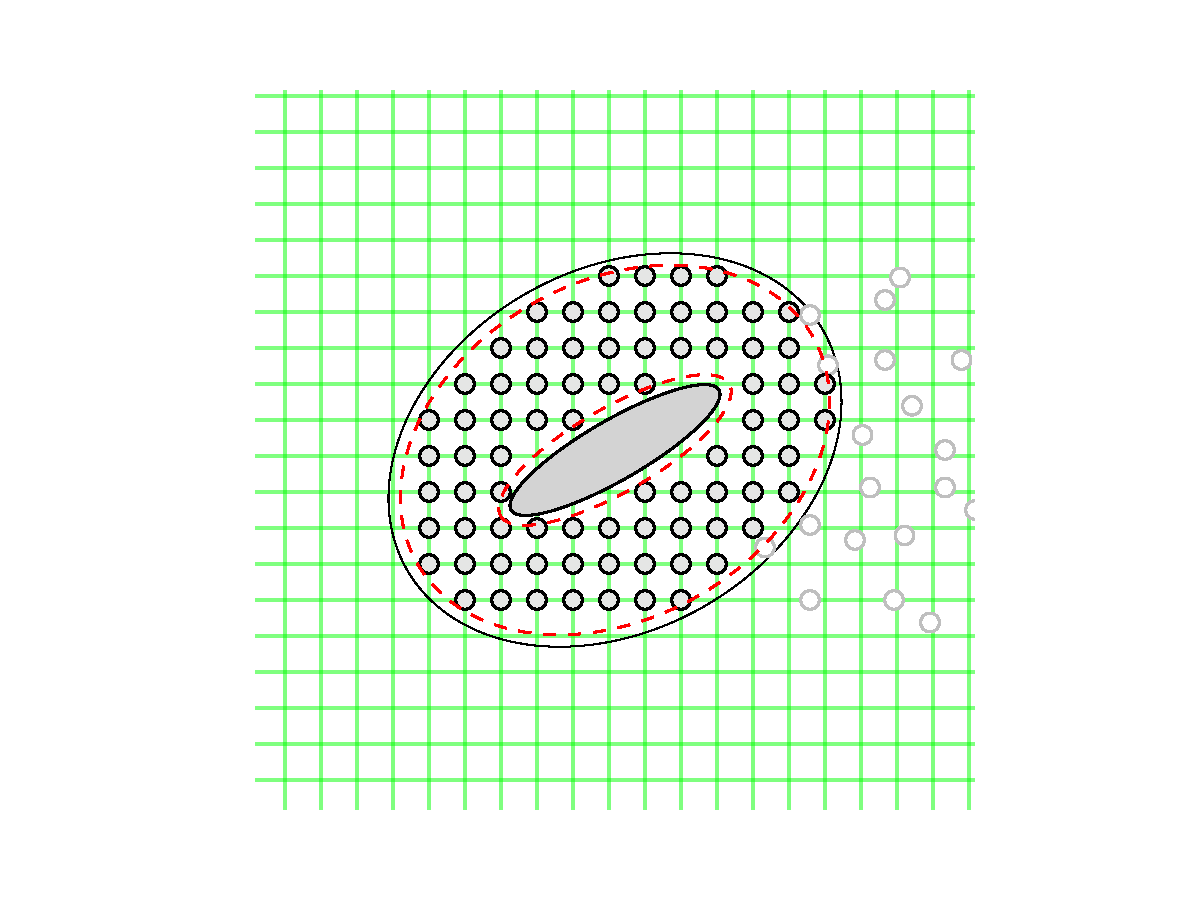
\includegraphics[trim=4.37cm 2.3cm 4.cm 2.cm, clip, width=0.5\linewidth]{./figures/hybrid/interpolation/ellipse/generatedParticles.pdf}
	\caption{Particles inside the interpolation domain $\Omega_{int}$ located at $\mathbf{x}_i$ coinciding the Lagrangian remeshing grid.}
	\label{fig:generatedParticles}
	\end{figure}

The procedures of generating zero-strength particles are as follows:
\begin{enumerate}
\item Generate zero-strength particles $\mathbf{x}_i$ inside the bounding box of the boundary polygon $\partial \Omega_{int}$, $\mathbf{x}_i \in \mathrm{BBOX}\{\partial \Omega_{int}\}$. The position of the particles $\mathbf{x}_i$ coincides with the global Lagrangian remeshing grid.
\item Perform a point-in-polygon test for the particles $\mathbf{x}_i$ to remove the particles outside the interpolation boundary $\partial \Omega_{int}$, and the particles inside the body $\Omega_{\mathrm{body}}$ and the vortex panel domain $\Omega_p$.
\end{enumerate}


\subsubsection*{Assign strengths}

	\begin{figure}[h]
	\centering
	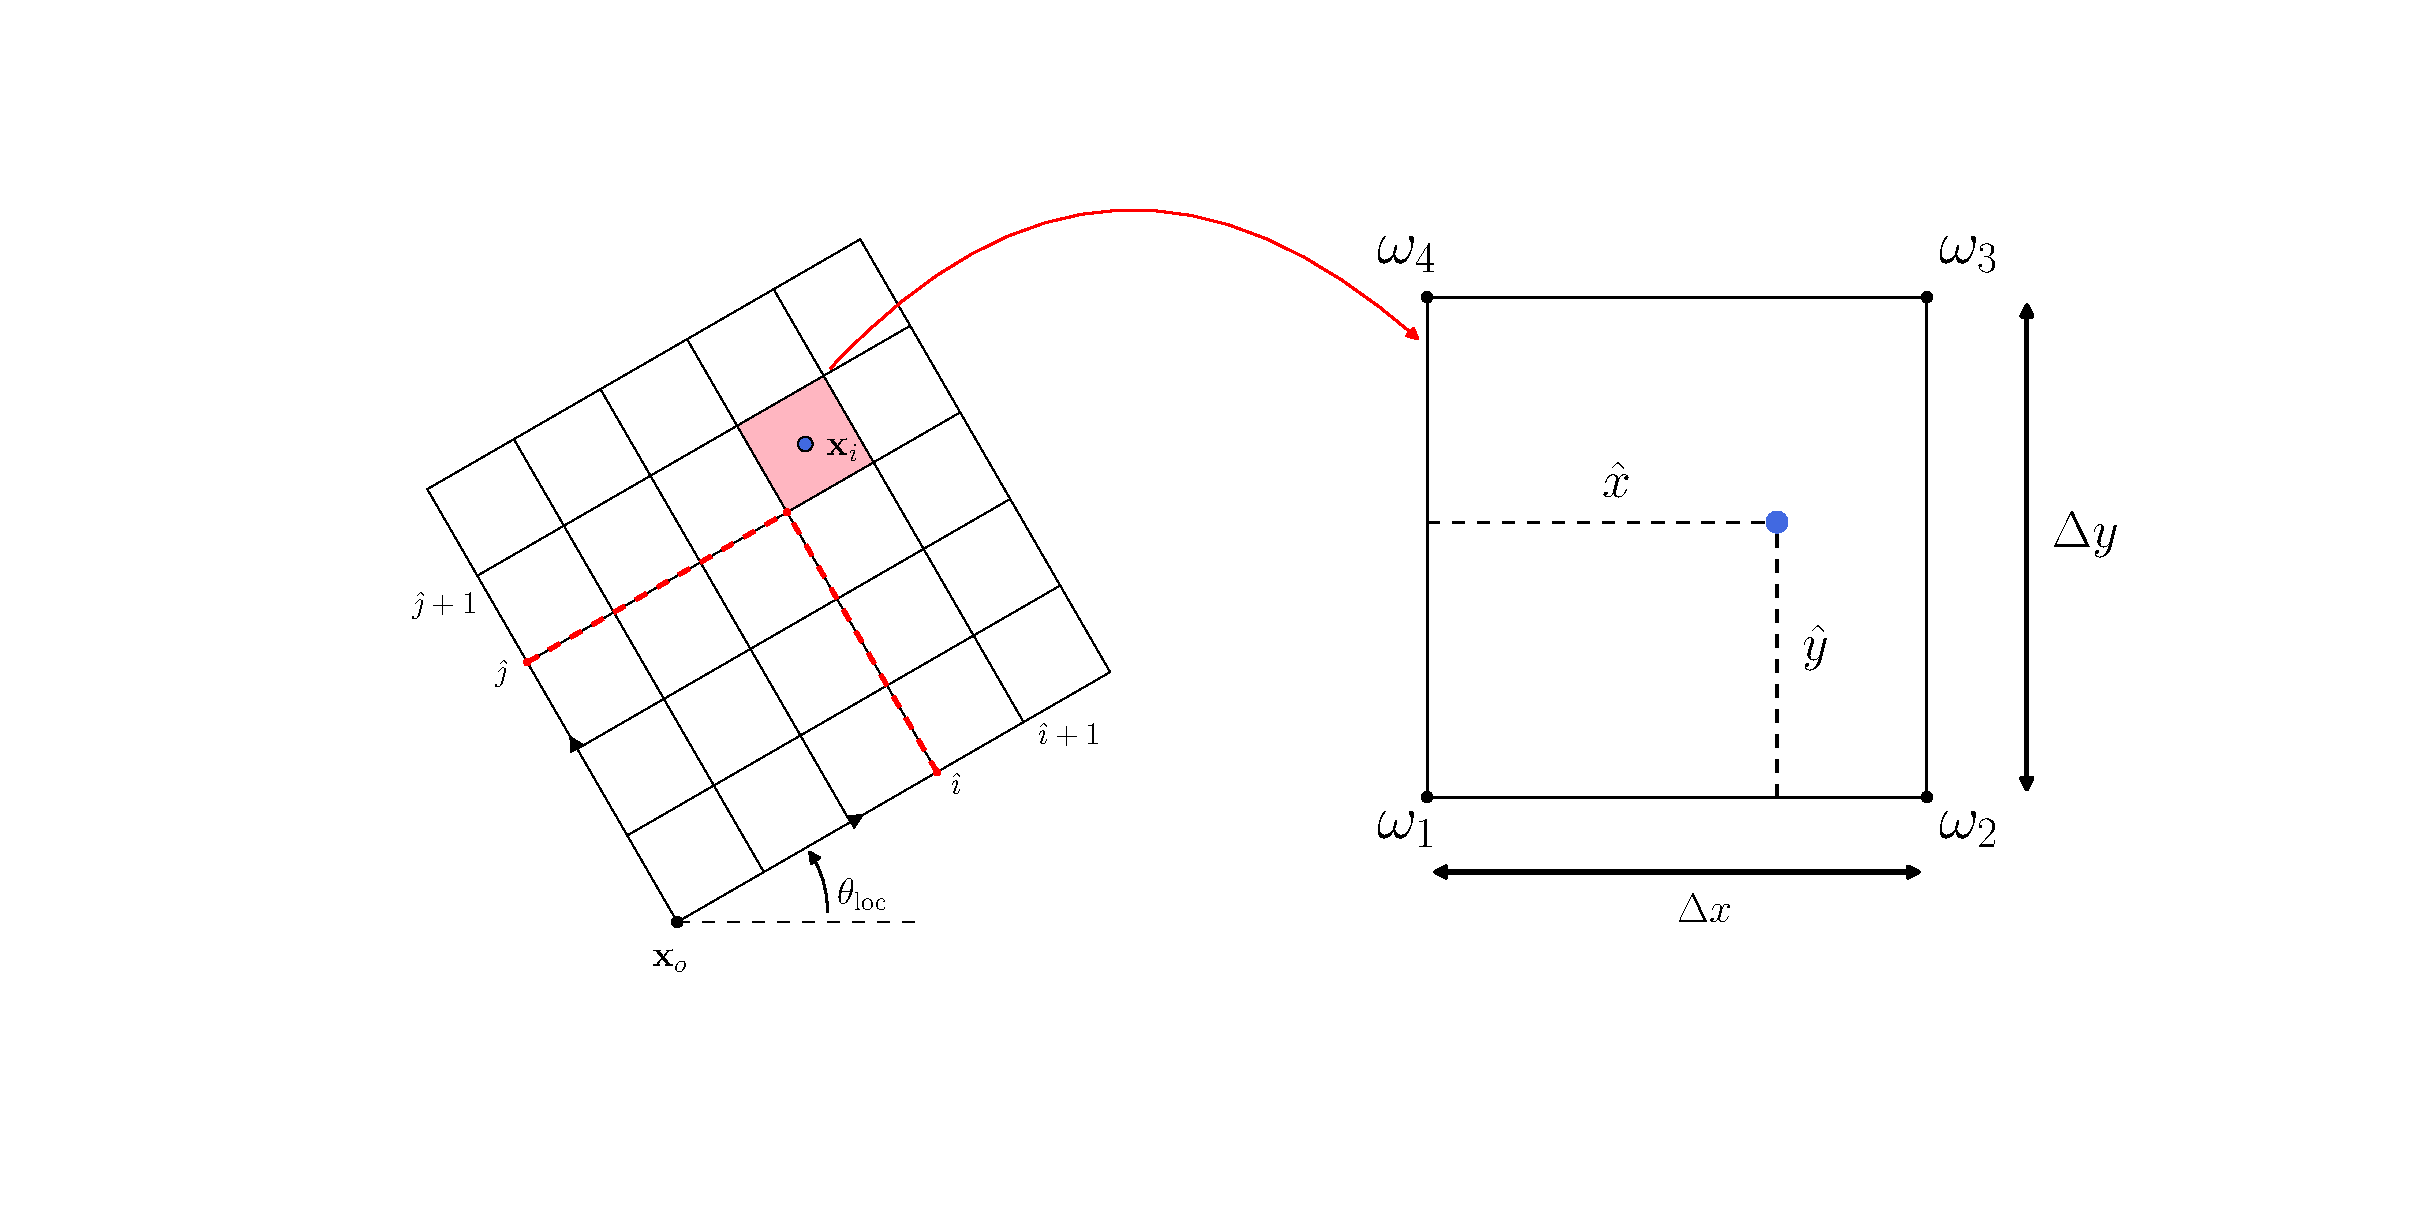
\includegraphics[trim=5.5cm 3.cm 4.5cm 3cm, clip, width=0.99\linewidth]{./figures/hybrid/interpolation/ellipse/interpolationManual.pdf}
	\caption{Interpolating the strengths from the structured grid $\mathbf{x}_{str}$ onto the vortex blobs $\mathbf{x}_i$ using a bilinear interpolation}
	\label{fig:interpolationManual}
	\end{figure}

The fourth sub-step of the correction is to assign the strengths to the newly generated particles in the interpolation domain $\Omega_{int}$. The strengths of the particles $\alpha_i$ is determined using the standard method,
\begin{equation}
\alpha(\mathbf{x}_i) = \hat{\omega}(\mathbf{x}_i) \cdot h^2,
\end{equation}
where the local circulation inside the area $h^2$ is assigned to the particle. As we have minimized the $h^2$ interpolation area such that the smoothing error caused the gaussian kernel is minimal. Therefore, to determine the strength of the particles inside the interpolation region, we simply require the vorticity $\hat{\omega}(\mathbf{x}_i)$ at the local $\mathbf{x}_i$. We have interpolated the finite element grid nodes onto a structure grid $\mathbf{x}_{str}$ which we can use to determine the vorticity at the position $\mathbf{x}_i$. We perform a bilinear interpolation of the vorticity from the nodes of the structure grid $\mathbf{x_i}$ onto particle at $\mathbf{x_i}$. Figure \ref{fig:interpolationManual} shows the algorithm for determining the strength. The particle (blue) is inside on of the cells of the grid (pink) bounded by 4 grid nodes $p_1 = \mathbf{x}_{i,j},\ p2  = \mathbf{x}_{i+1,j}, p3 = \mathbf{x}_{i+1,j+1}$ and $ p_4 = \mathbf{x}_{i,j+1}$, defined in the anti-clockwise direction. The bilinear interpolation of the vorticity becomes,
	\begin{equation}
	\hat{\omega}(\mathbf{x}_i) = \sum_{k=1}^4 W_k\cdot \omega_k
	\end{equation}
where $\omega_k, w_k \mapsto p_k$. The interpolation weights $w_k$ are defined as 
	\begin{equation}
	\begin{aligned}
	w_1 &= \frac{(\hat{x} - \Delta x )(\hat{y}-\Delta y)}{\Delta x \Delta y}\\
	w_2 &= \frac{-\hat{x}(\hat{y}-\Delta y)}{\Delta x \Delta y}\\
	w_3 &= \frac{\hat{x} \hat{y}}{\Delta x \Delta y}\\
	w_4 &= \frac{-\hat{y}(\hat{x} - \Delta x )}{\Delta x \Delta y}
	\end{aligned}
	\end{equation}
where the cell of the structured grid has dimension $[\Delta x, \Delta y]$ and the coordinates of the blobs are normalized such that, the vortex blobs is located at $0\leqslant\hat{x}\leqslant\Delta x$ and $0\leqslant\hat{y}\leqslant\Delta y$.
	
	\begin{figure}[h]
	\centering
	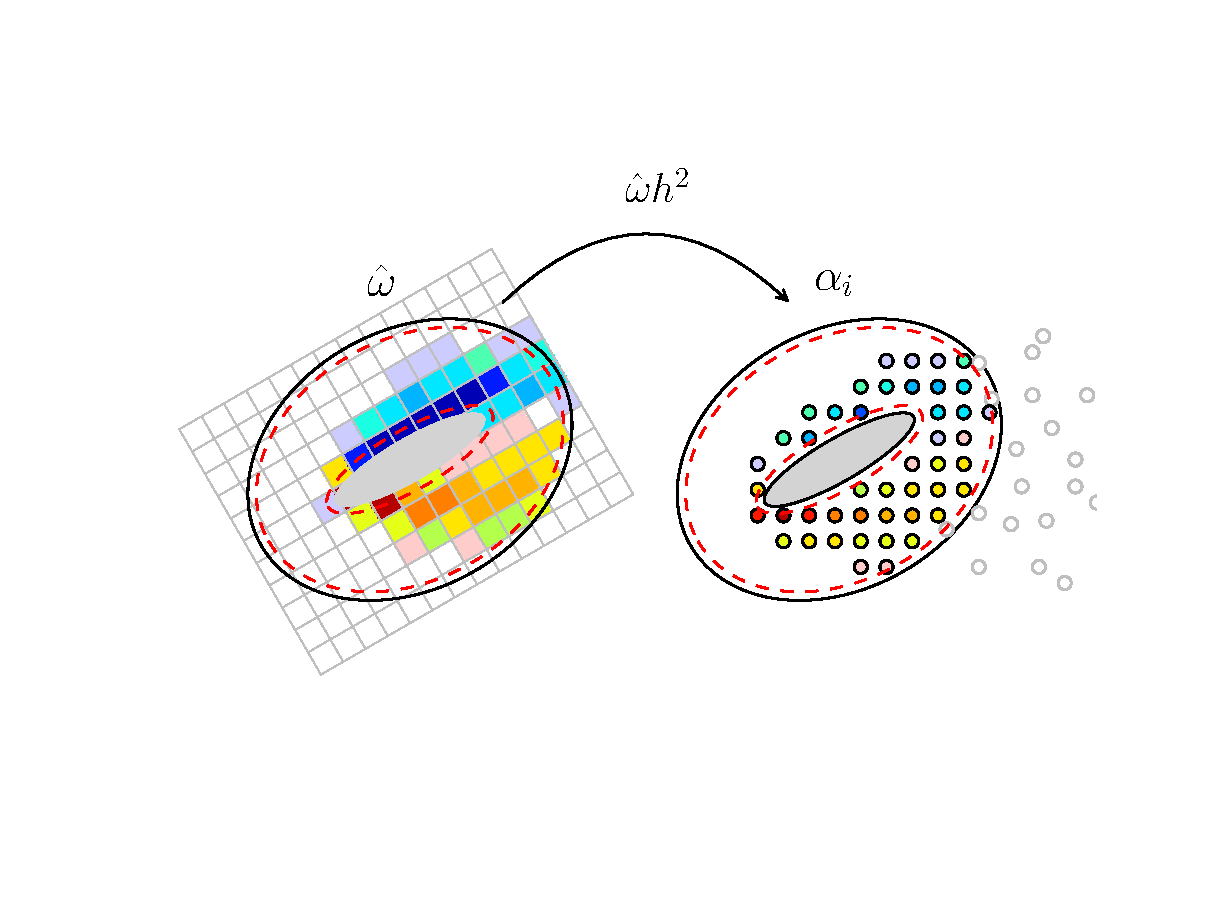
\includegraphics[trim=2.55cm 3.35cm 2.05cm 2.5cm, clip, width=0.9\linewidth]{./figures/hybrid/interpolation/ellipse/interpolation_StructuredGrid2Blobs.pdf}
	\caption{Interpolated strengths $\alpha_i$ from the structured grid $\mathbf{x}_{str}$ using bilinear interpolation.}
	\label{fig:interpolation_StructuredGrid2Blobs}
	\end{figure}
	

\subsubsection*{Conserve circulation}

The fifth and the final step of correcting the Lagrangian filed is to ensure that the we have to ensure that circulation is conserved. Two main source of errors for the conservation of circulation is the vorticity at the solid wall, and the vorticity field interpolation error.

The vorticity at the solid was not transfered to particles because the gaussian kernels cannot efficiently represent the singular distribution. However, we cannot simply neglect this distribution and therefore we use the vortex panels to represent this. The vortex panels are ideal as they can efficiently describe such wall bounded vorticity. To ensure the Lagrangian solver ensure conservation of circulation, we can prescribe the total bounded circulation on the panels.

The second error is the vorticity field interpolation error. The steps taken above does not satisfy conservation of circulation, therefore we should check that circulation is conserved. Assuming that we are dealing with a typical fluid flow with initial total circulation $\Gamma_0 = 0$, then according to Kelvin's circulation theorem, we require that at all times,
\begin{equation}
\Gamma_{panels} + \Gamma_{blobs} = 0.
\end{equation}

Thus, to ensure that the circulation is conserved, we have to solve for the no-slip panels such that the total circulation is zero. However, when we are dealing with multiple bodies, we have to formulate the equality in a different manner. We have to define two regions of the flow, domain where Eulerian solution is used, $\Omega_{inside} : \Omega_{body} \cup \Omega_p \cup \Omega_{int}$, and domain where Lagrangian solution is used $\Omega_{outside}: \Omega_L \backslash Omega_{inside}$. Figure \ref{}, depicts the two regions.

The total Lagrangian circulation now becomes,
\begin{equation}
\Gamma_{b,o}, \Gamma_{b,i} + \Gamma_p = 0
\end{equation}
where $\Gamma_{b,o}$ is the total circulation in the domain $\Omega_{outside}$, and $\Gamma_{b,i}+\Gamma_p$ is the total circulation in the domain $\Omega_{inside}$. Due to the correction algorithm, we require that the Lagrangian solutions in the domain $\Omega_{inside}$ matches the Eulerian solution. Therefore, we have the equality,
\begin{equation}
\Gamma_{Eulerian,i} = \Gamma_{b,i} + \Gamma_p,
\end{equation}
where $\Gamma_{Eulerian,i}$ total circulation from the Eulerian solution in the domain $\Omega_{Eulerian} \cap \Omega_{inside}$. Thus, the net strengths of the panels becomes,
\begin{equation}
\Gamma_p = \Gamma_{Eulerian,i} - \Gamma_{b,i}.
\end{equation}

In an ideal world, we would have $\Gamma_{Eulerian,i} + \Gamma_{b,o} = 0$, however as we have a slight error in the coupling scheme, due to the smoothing error, we will a small error in the total circulation $\epsilon_{\Gamma}$,
\begin{equation}
\Gamma_{Eulerian,i} + \Gamma_{b,o} = \epsilon_{\Gamma}.
\end{equation}
The simplest approach to remove this error is to modify the new generated blobs $\Gamma_{b,i}$ such that the total circulation $\Gamma=0$. This error is divided to all the new blobs equally,
\begin{equation}
\Gamma_{b,i}^{new} = \Gamma_{b,i} - \frac{\epsilon_{\Gamma}}{N_{b,i}},
\end{equation}
where $N_{b,i}$ is the total number of blobs generated inside the interpolation region $\Omega_{int}$.
\section{Evolution of the Lagrangian solution}
% - Advance lagrangian solution, Chapter lagrangian explains the algorithm

We have corrected the near-region solution of the Lagrangian domain $\Omega_L \cap \Omega_E$ with solution obtained from the Eulerian solver. Furthermore, we have solved the vortex panels such that: (a) it conserves the total circulation, and (b) it ensure the no-through/no-slip boundary condition. With the initial conditions provided at $t_n$, we can use the algorithms described in chapter \ref{ch:lagrangian}, to evolve the Lagrangian solution from $t_n$ to $t_{n+1}$. We can summarize the several features of the Lagrangian solver as follows:
\begin{itemize}
\item A $4^{\mathrm{th}}$-order Runge-Kutta method is used to time march the vorticity field from $t_n$ to $t_{n}+1$.
\item The Lagrangian solver has a convection time step size $\Delta t_c = t_{n+1}-t_n$.
\item We use Tutty's diffusion scheme such that the diffusion time step size $\Delta t_d = \Delta t_c$. Tutty's diffusion scheme is used in the majority of the cases as it is more versatile as it enables us to diffuse with convection ensure well represented vorticity field at every time $t$.
\item The strengths of the vortex panels $\gamma_i$ remains constant during $t_n$ and $t_{n+1}$. This is derived from the assumption that the change in the total circulation in domain $\Omega_p$ is small during $t_n$ and $t_{n+1}$.
\end{itemize}


\section{Evolution of the Eulerian solution}
% - Boundary conditions, all dirichlet from lagrangian

Once we have evolved the Lagrangian solution from $t_n$ to $t_{n+1}$, we can determine the boundary conditions for the Eulerian domain for $t_{n+1}$. In chapter \ref{ch:eulerian}, we have determined that to evolve the Eulerian solution, we require: (a) the initial velocity $\mathbf{u}$ and pressure $p$ distribution at $t_n$, and (b) the Dirichlet velocity boundary condition $\mathbf{u}$ at the boundary $\partial \Omega_E$ at the final step $t_{n+1}$.

\subsection{Dirichlet boundary conditions}

We can determine the Dirichlet velocity boundary condition at the Eulerian boundary $\partial \Omega_E$ from the Lagrangian vorticity field $\omega$ at $t_{n+1}$. In section \ref{}, we derived that the discrete mollifed velocity field of the vortex blobs. So, the velocity at the Eulerian boundary is given an,
\begin{equation}
\mathbf{u}(\mathbf{x}_{bdry},t_{n+1}) = \sum_p \mathbf{K}_{\sigma}[\mathbf{x}_{bdry} - \mathbf{x}_p(t_{n+1})]\alpha_p(t_{n+1}),
\end{equation}
where $\mathbf{x}_{bdrt}$ are the nodal coordinates of the Eulerian dirichlet boundary $\partial \Omega_E$, as shown in figure \ref{}.

\subsection{Multi-step evolution}
% Evolution, neglect the pressure b.c, and evolve the problem
% sub
	\begin{figure}[t]
	\centering
	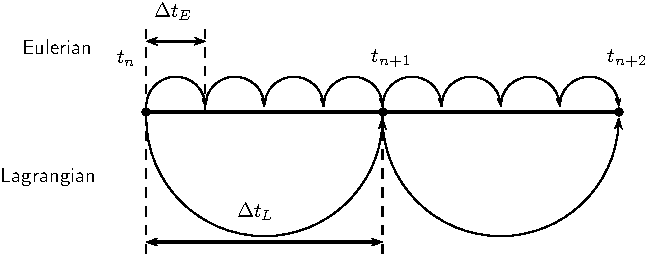
\includegraphics[width=0.7\linewidth]{./figures/eulerian/multiStep-crop.pdf}
	\caption{Eulerian multi-stepping to match the lagrangian $\Delta t_L$. The figures shows $\Delta t_L = 4 \Delta t_E$ and required $k_E = 4$ iterations to time march from $t_n$ to $t_{n+1}$.}
	\label{fig:multiStep}
	\end{figure}	

When coupling the Eulerian solver with the Lagrangian solver, we will see that the Eulerian time step size $\Delta t_E \leqslant \Delta t_L$. This is also the main benefit of the domain decomposition such that the wake region can be evolved with less time steps. So to reach the time $t_{n+1}$, we will have to perform $k_E$ Eulerian sub-steps to reach the Lagrangian step, 
\begin{equation}
t_{k} = t_n + k\Delta t_E,
\end{equation}
where $k = 1,...,k_E=\frac{t_{n+1}-t_{n}}{\Delta t_E}$. Figure \ref{fig:multiStep} depicts the multi-stepping of the Eulerian solution from $t_n$ to $t_{n+1}$ to match the lagrangian time. As, the Eulerian solver requires boundary condition at each sub-step, we have to perform a interpolation of the boundary conditions for each sub-step $t_k$. A linear interpolation of the boundary condition is given as,
\begin{equation}
\mathbf{u}(t_k) = \mathbf{u}(t_n) + k \Delta \mathbf{u}
\end{equation},
where $\Delta \mathbf{u} = \frac{\mathbf{u}(t_n+1)-\mathbf{u}(t_n)}{k_E}$. We can summarized the feature of the evolution of the Eulerian solution as follows:
\begin{itemize}
\item A $1^st$ order Forward Euler time-marching scheme is used to evolution the Eulerian solution from $t_n$ to $t_k$.
\item The solution is evolved $k_E$ steps to reach $t_{n+1}$.
\end{itemize}

\section{Introduction to pHyFlow: Hybrid solver}

We have implemented the algorithms described in chapter \ref{ch:lagrangian}, \ref{ch:eulerian}, and \ref{ch:hybrid} into \texttt{pHyFlow}, an acronym for  python Hybrid Flow solver. \texttt{pHyFlow} functions a computational fluid dynamics library for python, that has implemented an Eulerian solver, and a Lagrangian solver (without vortex diffusion of panels), which can be used as a standalone solver, or can be coupled together to make the Hybrid solver. 

The features of \texttt{pHyFlow} can be summarized as follows:
\begin{itemize}
\item \texttt{pHyFlow} is a hybrid flow solver that uses Hybrid Eulerian-Lagrangian Vortex Particle Method to couple the Navier-Stokes grid solver and a vortex blob solver.
\item The algorithms are written in \python, \textsc{Cython}, C, C++, and CUDA C/C++. All the high-level algorithms such as definition of the problem, coupling of the solver, convection and diffusion of the problem is perform in \python. The low-level algorithms such as remeshing kernel and the saving routine are written in the computationally efficient languages \textsc{Cython}, C, and C++. The parallelizable routine such as calculation of the induced velocity is written in CUDA C/C++ for the NVIDIA GPU.
\item \texttt{pHyFlow} uses several open-source libraries: FEniCS, Fenicstools, Scipy, Numpy, mpi4py, pyUblas, for performing the calculations; PyVTK, H5py, Matplotlib for plotting and efficient data storage.
\item \texttt{pHyFlow} is maintained, and is available at the bitbucket online repositiory\\ \texttt{https://bitbucket.org/apalha/phyflow2.0}.
\end{itemize}


\subsection{Program structure}

\begin{figure}[p]
\centering
\begin{tikzpicture}[%
  grow via three points={one child at (0.5,-0.7) and
  two children at (0.5,-0.7) and (0.5,-1.4)},
  edge from parent path={(\tikzparentnode.south) |- (\tikzchildnode.west)}]
  \node {\texttt{pHyFlow}}
    child {node [module] {\texttt{IO}}
   		child {node [class] {\texttt{File}}}
   	%child {node {\texttt{cpp}}}  	
    }
    child [missing] {}    
    child {node [module] {\texttt{aux}}
   		%child {node {\texttt{File}}}
   	%child {node {\texttt{cpp}}}  	
    } 
    child {node [module] {\texttt{blobs}}
		child {node [class] {\texttt{Blobs}}}
		child {node [module] {\texttt{base}}}  	
		child {node [script] {\texttt{blobOptions}}}  	
    }    
    child [missing] {}				
    child [missing] {}				
    child [missing] {}    			
    child { node [module] {\texttt{cpp}}
		child {node [module] {\texttt{blobs}}}
		child {node [module] {\texttt{panels}}}
    	}
    child [missing] {}	
    child [missing] {}    			
    child { node [module] {\texttt{eulerian}}
		child {node [class] {\texttt{EulerianSolver}}}
		child {node [module] {\texttt{base}}}
		child {node [script] {\texttt{eulerianOptions}}}
    	}
    child [missing] {}				
    child [missing] {}	
    child [missing] {}    
    child { node [module] {\texttt{hybrid}}
		child {node [class]{\texttt{HybridSolver}}}
		child {node [module] {\texttt{base}}}
		child {node [script] {\texttt{hybridOptions}}}
    	}
    child [missing] {}					
    child [missing] {}	
    child [missing] {}    
    child { node [module] {\texttt{lagrangian}}
		child {node [class] {\texttt{LagrangianSolver}}}
		child {node [module] {\texttt{base}}}
		child {node [script] {\texttt{lagrangianOptions}}}
    	}
    child [missing] {}				
    child [missing] {}	       
    child [missing] {}	
    child { node [module] {\texttt{panels}}
		child {node [class] {\texttt{Panels}}}
		child {node [module] {\texttt{base}}}
		child {node [script] {\texttt{panelOptions}}}
    	};
\end{tikzpicture}
\caption{Flowchart of the \texttt{pHyFlow} library structured into \mybox[fill=orange!50!red!50!white]{modules}, \mybox[fill=yellow!20]{option} script files, and \mybox[fill=blue!20]{classes}.}
\label{fig:tikz_pHyFlowStructure}
\end{figure}



The \texttt{pHyFlow} library serves as a computing environment for \python programming language, where one could solve the hybrid flow problems. To achieve this, we have implemented an Eulerian solver, and a Lagrangian solver (without panel diffusion scheme), which can be used as a standalone solver for verification and validation. The \texttt{pHyFlow} library is structured into several modules, categorized by their purposes. In each \texttt{module}, we defined a \texttt{class} that handles the functions in the module. To add flexibility in computation, we added an option file where the user change the solver options. Figure \ref{fig:tikz_pHyFlowStructure} shows the structure of the \texttt{pHyFlow} library, classified using a color code. The structure of the \texttt{pHyFlow} is as follows:

\begin{itemize}
\item \texttt{IO}: The module that contains all the input/output function for saving and plotting data. The \texttt{File} class handles the functions of the \texttt{IO} module.
\item \texttt{aux}: The module that contains all the auxiliary function of the library.
\item \texttt{cpp}: The module that contains all the low-level compiled function that has been wrapped using binding generator for the use in python. The two main low-level computations where induced velocity calculations for vortex blobs and vortex panels, and remeshing for the vortex blobs.
\item \texttt{blobs}: The module that contains all the vortex blob operations. The module contains the class \texttt{Blobs}, an the vortex blob solver object handling the all the vortex blobs operations.
\item \texttt{panels}: The module that contains all the vortex panel operations and wrapped in the class \texttt{Panels}, an the Panel method solver object.
\item \texttt{eulerian}: The module that contains all the Navier-Stokes grid operations and wrapped in \texttt{EulerianSolver}, the class containing all the high-level function for defining and managing the Eulerian solver.
\item \texttt{lagrangian}: The module that contains all the vortex blob and vortex panel coupling function and wrapped in \texttt{LagrangianSolver}, the class containing all the high-level function for managing the Lagrangian solver.
\end{itemize}


This is the main structure of the \texttt{pHyFlow} library. However, this is structured such that one could employ the library any general simulation purposes (hybrid, and non-hybrid simulation), where one could use a single module of \texttt{pHyFlow} library such a full potential flow problem with only vortex panels, or full grid problem using the Eulerian solver. 

\subsubsection{Hybrid class Hierarchy}

The hybrid module relies on the functions of the Lagrangian module and the Eulerian module. The Lagrangian module however requires the function of vortex blob module and the vortex panel module. Therefore, the Hierarchy of the Hybrid class is defined by figure \ref{fig:tikz_hybridStructure}. 

\begin{figure}[h]
\centering
\begin{tikzpicture}[%
  grow via three points={one child at (0.5,-0.7) and
  two children at (0.5,-0.7) and (0.5,-1.4)},
  edge from parent path={(\tikzparentnode.south) |- (\tikzchildnode.west)}]
  \node [class] {\texttt{hybrid}}
    child {node [class] {\texttt{Lagrangian}}
   		child {node [class] {\texttt{Blobs}}}
   		child {node [class] {\texttt{Panels}}}
    }
    child [missing] {}    
    child [missing] {}    
    child {node [class] {\texttt{Eulerian}}};
\end{tikzpicture}
\caption{Flowchart of the \texttt{HybridSolver}}
\label{fig:tikz_hybridStructure}
\end{figure}

We use a bottom-up approach to construct the \texttt{hybrid} class, starting the lower-level classes: \texttt{Blobs}, \texttt{Panels} and then constructing the mid-level classes: \texttt{Lagrangian}, and \texttt{Eulerian}, and finally constructing the high-level class. The procedure of constructing the hybrid class is as follows:
\begin{enumerate}
\item Define the \texttt{Blobs} class using the vorticity field parameters, the vortex blob parameters, time step parameters, and population control parameters. \\\\
Define the \texttt{Panels} class using panel geometry parameters.
\item Define \texttt{Lagrangian} class using the vortex blob class \texttt{Blobs} and the vortex panel class \texttt{Panels}.\\\\
Define \texttt{Eulerian} using the geometry mesh file, interpolation probe grid parameters, and the fluid parameters.
\item Define \texttt{Hybrid} using the lagrangian solver class \texttt{Lagrangian}, the Eulerian solver class \texttt{Eulerian} and the interpolation parameters.
\end{enumerate}

The detailed description of the Hybrid class Hierarchy is shown in appendix \ref{app:Code}.



%
%\section{Particle-Grid Coupling techniques}
%% Multiple ways of coupling , VIC, domain decomposition technique
%\subsection{Vortex in Cell method}
%
%\subsection{Particle-Grid domain decomposition methods}
%
%\section{Vortex diffusion methods}
%
%\subsection{Random walk method}
%\subsection{Core expansion method}
%\subsection{Particle-Strength Exchange}
%\subsection{Modified interpolation kernel for diffusion}
%
%\section{Simulation acceleration techniques}
%
%\subsection{Fast multi-pole Method}
%
%\subsection{Parallel computation in GPU}

%\section{Former Work}
%\label{sec:FormerWork}
%
%\subsection{Overview of the Work}
%\label{subsec:OverviewoftheWork}

%\section{Purpose of further research}

%%%%%%%%%%%%%%%%%%%%%%%%%%%%%%%%%%%%%%%%%%%%%%%%%%%%%%%%%%%%%%%%%%%%
%\nomenclature[ak]{$K$}{Kelvin (temperature)}
%\nomenclature[ar]{rpm}{Revolutions per minute (frequency)}
%\nomenclature[ac]{CO}{Carbon Monoxide}
%\nomenclature[ac]{CRM}{Chemical Reaction Modelling}
%\nomenclature[ah]{H2}{Molecular hydrogen}
%\nomenclature[ag]{GSP}{Gas Turbine Simulation Program (Software)}
%\nomenclature[rr]{$\rho$}{Density \nomunit{[$kg/{m^3}$]}}
%\nomenclature[sm]{$\dot{m}$}{Mass flow rate \nomunit{[$kg/s$]}}
%\nomenclature[ab]{bar}{Pressure}

%\nomenclature[rr]{$Re$}{Reynolds number \nomunit{[-]}}
%\nomenclature[rw]{$M$}{Mach number \nomunit{[-]}}
%\nomenclature[rw]{$\mu$}{Dynamic viscosity of air \nomunit{[$kg/{s \cdot m}$]}}